%-----------------------------------------------------------------------------
%
%               Template for sigplanconf LaTeX Class
%
% Name:         sigplanconf-template.tex
%
% Purpose:      A template for sigplanconf.cls, which is a LaTeX 2e class
%               file for SIGPLAN conference proceedings.
%
% Author:       Paul C. Anagnostopoulos
%               Windfall Software
%               978 371-2316
%               paul@windfall.com
%
% Created:      15 February 2005
%
%-----------------------------------------------------------------------------


\documentclass[preprint]{sigplanconf}

% The following \documentclass options may be useful:
%
% 10pt          To set in 10-point type instead of 9-point.
% 11pt          To set in 11-point type instead of 9-point.
% authoryear    To obtain author/year citation style instead of numeric.

\usepackage{ifthen}
\usepackage{fancyvrb}
\usepackage{color}
\usepackage{ulem}
\usepackage{xspace}
\usepackage{epsfig}
\usepackage{amssymb}
\usepackage{amsmath}
\usepackage{amsfonts}
\usepackage[utf8]{inputenc}
\usepackage{setspace}

\usepackage{listings}

\usepackage[T1]{fontenc}
\usepackage{setspace}
\usepackage{listings}
\usepackage{beramono}


\definecolor{gray}{rgb}{0.3,0.3,0.3}

\lstset{
  basicstyle=\setstretch{1.05}\ttfamily\footnotesize,
  language=Python,
  keywordstyle=\bfseries,
  stringstyle=\color{blue},
  commentstyle=\color{gray}\textit,
  fancyvrb=true,
  showstringspaces=false,
  %keywords={def,while,if,elif,return,class,get,set,new,guard_class}
  numberstyle = \tiny,
  numbersep = -20pt,
}


\newboolean{showcomments}
\setboolean{showcomments}{true}
\ifthenelse{\boolean{showcomments}}
  {\newcommand{\nb}[2]{
    \fbox{\bfseries\sffamily\scriptsize#1}
    {\sf\small$\blacktriangleright$\textit{#2}$\blacktriangleleft$}
   }
   \newcommand{\version}{\emph{\scriptsize$-$Id: main.tex 19055 2008-06-05 11:20:31Z cfbolz $-$}}
  }
  {\newcommand{\nb}[2]{}
   \newcommand{\version}{}
  }

\newcommand\cfbolz[1]{\nb{CFB}{#1}}
\newcommand\arigo[1]{\nb{AR}{#1}}
\newcommand\fijal[1]{\nb{FIJAL}{#1}}
\newcommand\david[1]{\nb{DAVID}{#1}}
\newcommand\anto[1]{\nb{ANTO}{#1}}
\newcommand\reva[1]{\nb{Reviewer 1}{#1}}
\newcommand\revb[1]{\nb{Reviewer 2}{#1}}
\newcommand\revc[1]{\nb{Reviewer 3}{#1}}
\newcommand{\commentout}[1]{}
\newcommand{\ignore}[1]{} % {{\tt \small ignore(#1)}}

\newcommand\ie{i.e.,\xspace}
\newcommand\eg{e.g.,\xspace}
\newcommand{\etal}{\emph{et al.}\xspace}

\normalem

\let\oldcite=\cite

\renewcommand\cite[1]{\ifthenelse{\equal{#1}{XXX}}{[citation~needed]}{\oldcite{#1}}}


\begin{document}

\conferenceinfo{IWTC '11}{XXX} 
\copyrightyear{2011} 
\copyrightdata{[to be supplied]} 

\titlebanner{draft}        % These are ignored unless
%\preprintfooter{short description of paper}   % 'preprint' option specified.

\title{Loop Invariant Code Motion in PyPy's Tracing JIT}
%\subtitle{Subtitle Text, if any}

\authorinfo{H\aa kan Ardö}
           {Centre for Mathematical Sciences, Lund University}
           {hakan@debian.org}
\authorinfo{Carl Friedrich Bolz}
           {Heinrich-Heine-Universität Düsseldorf}
           {cfbolz@gmx.de}
\authorinfo{Maciej Fijałkowski}
           {Affiliation2}
           {fijall@gmail.com}

\maketitle

\begin{abstract}
This is the text of the abstract.
\end{abstract}

\category{D.3.4}{Programming Languages}{Processors}[code generation,
incremental compilers, interpreters, run-time environments]

\terms
Languages, Performance, Experimentation

\keywords{Tracing JIT, Optimization, Loop-Invariant Code Motion}

\section{Introduction}

One of the advantages that tracing JIT compilers have above traditional
method-based
JITs is that their optimizers are much easier to write. Because a tracing JIT
produces only linear pieces of code without control flow joins, many
optimization passes on traces can have a very simple structure. They often
consist of one forward pass replacing operations by simpler ones or even
discarding them as they walk along it. This makes
optimization of traces very similar to symbolic execution. Also, many
difficult problems in traditional optimizers become tractable if the optimizer
does not need to deal with control flow merges.

One disadvantage of this simplicity is that such simple forward-passing
optimizers ignore the only bit of control flow they have available, which is
the fact that most traces actually represent loops. Making use of this
information is necessary to perform optimizations that take the whole loop into
account, such as loop-invariant code
motion or optimizations that improve across several iterations of the loop.
Having to deal with this property of traces complicates the optimization passes,
as a more global view of a trace needs to be considered when optimizing.

In this paper we want to address this problem by proposing a simple scheme that
makes it possible to turn simple optimizations using one forward pass into
optimizations that can do loop invariant code motion and similar loop-aware
improvements. Using this scheme one does not need to change the underlying
optimization much to get these advantages.

XXX "bridge" is not a standard term

XXX loop peeling does a lot more than loop-invariant code motion
% take this loop as an example:
% [i1, i2]
% i3 = i1 + 1
% i4 = i2 + 1
% escape(i4)
% jump(i2, i3)
% none of the operations is loop-invariant, but loop peeling will still remove the second addition

\subsection{Running Example}
\label{sub:example}

For the purpose of this paper, we are going to use a tiny interpreter for a dynamic language with
 a very simple object
model, that just supports an integer and a float type (this example has been taken from a previous paper \cite{bolz_allocation_2011}). The objects support only
two operations, \lstinline{add}, which adds two objects (promoting ints to floats in a
mixed addition). The implementation of \lstinline{add} uses classical Smalltalk-like
double-dispatching.
%These classes could be part of the implementation of a very
%simple interpreter written in RPython.
The classes can be seen in
Figure~\ref{fig:objmodel} (written in RPython).

\begin{figure}
\begin{lstlisting}[mathescape,basicstyle=\setstretch{1.05}\ttfamily\scriptsize]
class Base(object):
   pass

class BoxedInteger(Base):
   def __init__(self, intval):
      self.intval = intval

   def add(self, other):
      return other.add__int(self.intval)

   def add__int(self, intother):
      return BoxedInteger(intother + self.intval)

   def add__float(self, floatother):
      floatvalue = floatother + float(self.intval)
      return BoxedFloat(floatvalue)


class BoxedFloat(Base):
   def __init__(self, floatval):
      self.floatval = floatval

   def add(self, other):
      return other.add__float(self.floatval)

   def add__int(self, intother):
      floatvalue = float(intother) + self.floatval
      return BoxedFloat(floatvalue)

   def add__float(self, floatother):
      return BoxedFloat(floatother + self.floatval)


def f(y):
   step = BoxedInteger(-1)
   while True:
      y = y.add(step)
\end{lstlisting}
\caption{An ``Interpreter'' for a Tiny Dynamic Language Written in RPython}
\label{fig:objmodel}
\end{figure}

Using these classes to implement arithmetic shows the basic problem of many
dynamic language implementations. All the numbers are instances of either
\lstinline{BoxedInteger} or \lstinline{BoxedFloat}, therefore they consume space on the
heap. Performing many arithmetic operations produces lots of garbage quickly,
putting pressure on the garbage collector. Using double dispatching to
implement the numeric tower needs two method calls per arithmetic operation,
which is costly due to the method dispatch.

Let us now consider a simple ``interpreter'' function \lstinline{f} that uses the
object model (see the bottom of Figure~\ref{fig:objmodel}).
Simply running this function is slow, because there are lots of virtual method
calls inside the loop, two for each
call to \lstinline{add}. These method calls need to check the type of the involved
objects every iteration. In addition, a lot of objects are created
when executing that loop, many of these objects are short-lived.
The actual computation that is performed by \lstinline{f} is simply a sequence of
float or integer additions (note that \lstinline{f} does not actually terminate,
but it is still instructive to look at the produced traces).


\begin{figure}
\begin{lstlisting}[mathescape,numbers = right,basicstyle=\setstretch{1.05}\ttfamily\scriptsize]
$l_0$($p_{0}$, $p_{1}$):
# inside f: y = y.add(step)
guard_class($p_{1}$, BoxedInteger)
    # inside BoxedInteger.add
    $i_{2}$ = get($p_{1}$, intval)
    guard_class($p_{0}$, BoxedInteger)
        # inside BoxedInteger.add__int
        $i_{3}$ = get($p_{0}$, intval)
        $i_{4}$ = $i_{2} + i_{3}$
        $p_{5}$ = new(BoxedInteger)
            # inside BoxedInteger.__init__
            set($p_{5}$, intval, $i_{4}$)
jump($l_0$, $p_{0}$, $p_{5}$)
\end{lstlisting}
\caption{An Unoptimized Trace of the Example Interpreter}
\label{fig:unopt-trace}
\end{figure}

If the function is executed using the tracing JIT, with \lstinline{y} being a
\lstinline{BoxedInteger}, the produced trace looks like the one of
Figure~\ref{fig:unopt-trace} (lines starting with a hash ``\#'' are comments).
The trace corresponds to one iteration of the while-loop in \lstinline{f}.

The operations in the trace are indented
corresponding to the stack level of the function that contains the traced
operation. The trace is in single-assignment form, meaning that each variable is
assigned a value exactly once. The arguments $p_0$ and $p_1$ of the loop correspond
to the live variables \lstinline{y} and \lstinline{res} in the while-loop of
the original function.

The label of the loop is $l_0$ and is used by the jump instruction to
identify it's jump target.

The operations in the trace correspond to the operations in the RPython program
in Figure~\ref{fig:objmodel}:

\begin{itemize}
    \item \lstinline{new} creates a new object.
    \item \lstinline{get} reads an attribute of an object.
    \item \lstinline{set} writes to an attribute of an object.
    \item \lstinline{guard_class} is a precise type check. It typically precedes
    an (inlined) method call and is followed by the trace of the called method.
    \item \lstinline{guard_true} checks that a boolean is true.
\end{itemize}

Method calls in the trace are preceded by a \lstinline{guard_class}
operation, to check that the class of the receiver is the same as the one that
was observed during tracing.\footnote{\lstinline{guard_class}
performs a precise
class check, not checking for subclasses.} These guards make the trace specific
to the situation where \lstinline{y} is really a \lstinline{BoxedInteger}. When
the trace is turned into machine code and afterwards executed with
\lstinline{BoxedFloat}, the
first \lstinline{guard_class} instruction will fail and execution will continue
using the interpreter.

\section{Trace Optimizations}

XXX make clear that the preamble is not necessarily the \emph{first} iteration
of a loop

Before the trace is passed to a backend compiling it into machine code
it needs to be optimized to achieve better performance.
The focus of this paper
is loop invariant code motion. The goal of that is to move as many
operations as possible out of the loop making them executed at most once
and not every iteration. This we propose to achieve by loop peeling. It
leaves the loop body intact, but prefixes it with one iteration of the
loop. This operation by itself will not achieve anything. But if it is
combined with other optimizations it can increase the effectiveness of
those optimizations. For many optimization of interest some care has
to be taken when they are combined with loop peeling. This is
described below by first explaining the loop peeling optimization
followed by a set of other optimizations and how they interact with
loop peeling.

\subsection{Loop Peeling}

\begin{figure}
\begin{center}
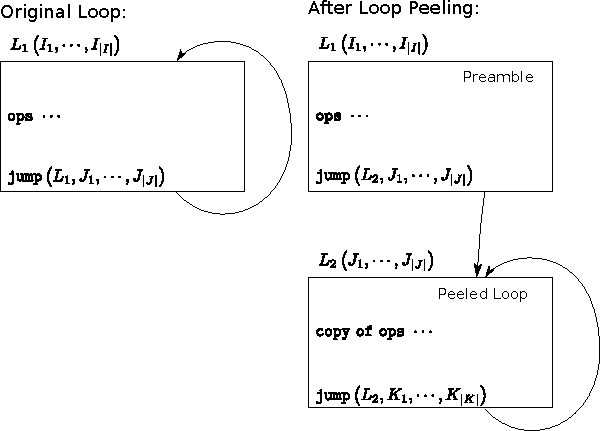
\includegraphics[scale=1]{figures/overview}
\end{center}
\end{figure}

XXX find reference

Loop peeling is achieved by appending a copy of the traced iteration at
the end of the loop. The copy  is inlined to make the two parts form a
consistent two iteration trace. 
The first part (called preamble) finishes with the jump the the second part
(called peeled loop). The second part ends up with the jump to itself. This way
the preamble will be executed only once while the peeled loop will
be used for every other iteration.
The trace from Figure~\ref{fig:unopt-trace} would after this operation become
the trace in Figure~\ref{fig:peeled-trace}. Line 1-13 shows the
preamble while line 15-27 shows the peeled loop.

\begin{figure}
\begin{lstlisting}[mathescape,numbers = right,basicstyle=\setstretch{1.05}\ttfamily\scriptsize]
$l_0$($p_{0}$, $p_{1}$):
# inside f: y = y.add(step)
guard_class($p_{1}$, BoxedInteger)
    # inside BoxedInteger.add
    $i_{2}$ = get($p_{1}$, intval)
    guard_class($p_{0}$, BoxedInteger)
        # inside BoxedInteger.add__int
        $i_{3}$ = get($p_{0}$, intval)
        $i_{4}$ = $i_{2}+i_{3}$
        $p_{5}$ = new(BoxedInteger)
            # inside BoxedInteger.__init__
            set($p_{5}$, intval, $i_{4}$)
jump($l_1$, $p_{0}$, $p_{5}$)

$l_1$($p_{0}$, $p_{5}$):
# inside f: y = y.add(step)
guard_class($p_{5}$, BoxedInteger)
    # inside BoxedInteger.add
    $i_{6}$ = get($p_{5}$, intval)
    guard_class($p_{0}$, BoxedInteger)
        # inside BoxedInteger.add__int
        $i_{7}$ = get($p_{0}$, intval)
        $i_{8}$ = $i_{6}+i_{7}$
        $p_{9}$ = new(BoxedInteger)
            # inside BoxedInteger.__init__
            set($p_{9}$, intval, $i_{8}$)
jump($l_1$, $p_{0}$, $p_{9}$)
\end{lstlisting}
\caption{A peeled trace of the Example Interpreter}
\label{fig:peeled-trace}
\end{figure}

When applying the following optimizations to this two-iteration trace
some care has to taken as to how the arguments of the two
\lstinline{jump} operations and the input arguments of the peeled loop are
treated. It has to be ensured that the peeled loop stays a proper
trace in the sense that the operations within it only operates on
variables that are either among its input arguments 
or produced within the peeled loop. To ensure this we need
to introduce a bit of formalism.

The original trace (prior to peeling) consists of three parts.
A vector of input
variables, $I=\left(I_1, I_2, \cdots, I_{|I|}\right)$, a list of non-
jump operations and a single
jump operation. The jump operation contains a vector of jump variables,
$J=\left(J_1, J_2, \cdots, J_{|J|}\right)$, that are passed as the input variables of the target loop. After
loop peeling there will be a second copy of this trace with input
variables equal to the jump arguments of the preamble, $J$, and jump
arguments $K$. Looking back at our example we have
\begin{equation}
  %\left\{
    \begin{array}{lcl}
      I &=& \left( p_0, p_1 \right) \\
      J &=& \left( p_0, p_5 \right) \\
      K &=& \left( p_0, p_9 \right) \\
    \end{array}
  %\right.
  .
\end{equation}
To construct the second iteration from the first we also need a
function $m$, mapping the variables of the preamble onto the
variables of the peeled loop. This function is constructed during the
inlining. It is initialized by mapping the input arguments, $I$, to
the jump arguments $J$,
\begin{equation}
  m\left(I_i\right) = J_i \ \text{for}\ i = 1, 2, \cdots |I| .
\end{equation}
In the example that means:

\begin{equation}
  %\left\{
    \begin{array}{lcl}
      m\left(p_0\right) &=& p_0 \\
      m\left(p_1\right) &=& p_5
    \end{array}
  %\right.
  .
\end{equation}

Each operation in the trace is inlined in order.
To inline an operation $v=\text{op}\left(A_1, A_2, \cdots, A_{|A|}\right)$
a new variable, $\hat v$ is introduced. The inlined operation will
produce $\hat v$ using
\begin{equation}
  \hat v = \text{op}\left(m\left(A_1\right), m\left(A_2\right), 
    \cdots, m\left(A_{|A|}\right)\right) . 
\end{equation}
Before the
next operation is inlined, $m$ is extend by assigning $m\left(v\right) = \hat
v$. For the example above, after all the operations have been inlined we have
\begin{equation}
  %\left\{
    \begin{array}{lcl}
      m\left(p_0\right) &=& p_0 \\
      m\left(p_1\right) &=& p_5 \\
      m\left(i_2\right) &=& i_6 \\
      m\left(i_3\right) &=& i_7 \\
      m\left(i_4\right) &=& i_8 \\
      m\left(p_5\right) &=& p_9 \\
    \end{array}
  %\right.
  .
\end{equation}

\subsection{Redundant Guard Removal}

XXX should we have a mention where in the previous papers those optimizations
are discussed? Is the previous XXX precisely about this?

No special concerns needs to be taken when implementing redundant
guard removal together with loop peeling. The guards from
the preamble might make the guards of the peeled loop
redundant and thus removed. Therefore the net effect of combining redundant
guard removal with loop peeling is that loop-invariant guards are moved out of the
loop. The peeled loop of the example reduces to

\begin{lstlisting}[mathescape,numbers = right,basicstyle=\setstretch{1.05}\ttfamily\scriptsize]
$l_1$($p_{0}$, $p_{5}$):
# inside f: y = y.add(step)
    # inside BoxedInteger.add
    $i_{6}$ = get($p_{5}$, intval)
        # inside BoxedInteger.add__int
        $i_{7}$ = get($p_{0}$, intval)
        $i_{8}$ = $i_{6}+i_{7}$
        $p_{9}$ = new(BoxedInteger)
            # inside BoxedInteger.__init__
            set($p_{9}$, intval, $i_{8}$)
jump($l_1$, $p_{0}$, $p_{9}$)
\end{lstlisting}

The guard on $p_5$ on line 17 of Figure~\ref{fig:unopt-trace} can be
removed since $p_5$ is allocated on line 10 with a known class. The
guard on $p_0$ on line 20 can be removed since it is identical to the
guard on line 6.

\subsection{Heap Caching}

XXX gcc calls this store-sinking and I'm sure there are some
references in the literature (none at hand though). This is a ``typical''
compiler optimization.

The objective of heap caching is to remove \lstinline{get} and
\lstinline{set} operations whose results can be deduced from previous
\lstinline{get} and \lstinline{set} operations. Exact details of the
process are outside the scope of this paper. We only consider the interaction
with loop peeling.

The issue at hand is to keep the peeled loop a proper
trace. Consider the \lstinline{get} operation on line 19 of
Figure~\ref{fig:unopt-trace}. The result of this operation can be
deduced to be $i_4$ from the \lstinline{set} operation on line
12. Also, the result of the \lstinline{get} operation on line 22 can
be deduced to be $i_3$ from the \lstinline{get} operation on line
8. The optimization will thus remove line 19 and 22 from the trace and
replace $i_6$ with $i_4$ and $i_7$ with $i_3$. 

After that, the peeled loop
will no longer be in SSA form as it operates on $i_3$ and $i_4$
which are not part of it. The solution is to extend the input
arguments, $J$, with those two variables. This will also extend the
jump arguments of the preamble, which is also $J$. 
Implicitly that also extends the jump arguments of the peeled loop, $K$,
since they are the inlined versions of $J$. For the example $I$ has to
be replaced by $\hat I$ which is formed as a concatenation of $I$ and
$\left(i_3, i_4\right)$. At the same time $K$ has to be replaced by
$\hat K$ which is formed as a concatenation of $K$ and 
$\left(m\left(i_3\right), m\left(i_4\right)\right) = \left(i_7, i_8\right)$. 
The variable $i_7$ will then be replaced by $i_3$ by the heap caching
optimization as it has removed the variable $i_7$. XXX: Maybe we should
replace $i_7=$get(...) with $i_7=i_3$ instead of removing it?

In general what is needed is for the heap optimizer is to keep track of
which variables from the preamble it reuses in the peeled loop.
It has to construct a vector of such variables $H$ which
can be used to update the input and jump arguments using
\begin{equation}
  \hat J = \left(J_1, J_2, \cdots, J_{|J|}, H_1, H_2, \cdots, H_{|H}\right)
  \label{eq:heap-inputargs}
\end{equation}
and
\begin{equation}
  \hat K = \left(K_1, K_2, \cdots, K_{|J|}, m(H_1), m(H_2), \cdots, m(H_{|H})\right)
  .
  \label{eq:heap-jumpargs}
\end{equation}
In the optimized trace $I$ is replaced by $\hat I$ and $K$ by $\hat
K$. The trace from Figure~\ref{fig:unopt-trace} will be optimized to:

\begin{lstlisting}[mathescape,numbers = right,basicstyle=\setstretch{1.05}\ttfamily\scriptsize]
$l_0$($p_{0}$, $p_{1}$):
# inside f: y = y.add(step)
guard_class($p_{1}$, BoxedInteger)
    # inside BoxedInteger.add
    $i_{2}$ = get($p_{1}$, intval)
    guard_class($p_{0}$, BoxedInteger)
        # inside BoxedInteger.add__int
        $i_{3}$ = get($p_{0}$, intval)
        $i_{4}$ = $i_{2}+i_{3}$
        $p_{5}$ = new(BoxedInteger)
            # inside BoxedInteger.__init__
            set($p_{5}$, intval, $i_{4}$)
jump($l_1$, $p_{0}$, $p_{5}$, $i_3$, $i_4$)

$l_1$($p_{0}$, $p_{5}$, $i_3$, $i_4$):
# inside f: y = y.add(step)
    # inside BoxedInteger.add
        # inside BoxedInteger.add__int
        $i_{8}$ = $i_{4}+i_{3}$
        $p_{9}$ = new(BoxedInteger)
            # inside BoxedInteger.__init__
            set($p_{9}$, intval, $i_{8}$)
jump($l_1$, $p_{0}$, $p_{9}$, $i_3$, $i_8$)
\end{lstlisting}

\subsection{Common Subexpression Elimination}
If a pure operation appears more than once in the trace with same input
arguments, it only needs be executed the first time and then the result
can be reused for all other appearances. When that is combined with loop
peeling, the single execution of the operation is placed in the
preamble. That is, loop invariant pure operations are moved out of the
loop. The interactions here are the same as in the previous
section. That is, a vector, $H$, of variables produced in the preamble
and used in the peeled loop needs to be constructed. Then the jump and
input arguments are updated according to
Equation~\ref{eq:heap-inputargs} and Equation~\ref{eq:heap-jumpargs}.

\subsection{Allocation Removals}
By using escape analysis it is possible to identify objects that are
allocated within the loop but never escape it. That is 
short lived objects with no references outside the loop. This
is performed by processing the operation in order and
optimistically removing every \lstinline{new} operation. Later on if
it is discovered that a reference to the object escapes the loop, the
\lstinline{new} operation is inserted at this point. All operations
(\lstinline{get} and \lstinline{set}) on the removed objects are also
removed and the optimizer needs to keep track of the value of all
used attributes of the object.

Consider again the original unoptimized trace of
Figure~\ref{fig:peeled-trace}. Line 10 contains the first
allocation. It is removed and $p_5$ is marked as virtual. This means
that it refers to an virtual object that was not yet been
(and might never be) allocated. Line 12 sets the \lstinline{intval}
attribute of $p_5$. This operation is also removed and the optimizer
registers that the attribute \lstinline{intval} of $p_5$ is $i_4$.

When the optimizer reaches line 13 it needs to construct the
arguments of the \lstinline{jump} operation, which contains the virtual
reference $p_5$. This can be achieved by exploding $p_5$ into it's
attributes. In this case there is only one attribute and it's value is
$i_4$, which means the $p_5$ is replaced with $i_4$ in the jump
arguments. 

In the general case, each virtual in the jump arguments is exploded into a
vector of variables containing the values of all registered attributes. If some
of the attributes are themselves virtuals they are recursively exploded
to make the vector contain only non-virtual variables. Some care has
to be taken to always place the attributes in the same order when
performing this explosion. Notation becomes somewhat simpler if also every non-
virtual variable of the jump arguments is exploded into a vector. This will
be a vector containing the original variable only. To summarize, for
every variable, $J_k$, of the original jump arguments, $J$, let
\begin{equation}
  \tilde J^{\left(k\right)} = \left\{
      \begin{array}{ll}
        \left(J_k\right)  & \text{if $J_k$ is not virtual} \\
        H^{\left(k\right)} & \text{if $J_k$ is virtual}
      \end{array}
  \right.
  ,
\end{equation}
where $H^{\left(k\right)}$ is a vector containing all non virtual
attributes of $J_k$. The arguments of the optimized \lstinline{jump}
operation are constructed as the concatenation all the $\tilde J^{\left(k\right)}$ vectors,
\begin{equation}
  \hat J = \left( 
    \begin{array}{cccc}
      \tilde J^{\left(1\right)} & \tilde J^{\left(2\right)} & \cdots &
      \tilde J^{\left(|J|\right)} \\
    \end{array}
  \right)      
  .
\end{equation}
and the arguments of the \lstinline{jump} operation of the peeled loop,
$K$, constructed by inlining $\hat J$,
\begin{equation}
  \hat K = \left(m\left(\hat J_1\right), m\left(\hat J_1\right), 
                 \cdots, m\left(\hat J_{|\hat J|}\right)\right)
  .
\end{equation}
In the optimized trace $I$ is replaced by $\hat I$ and $K$ by $\hat
K$. The trace from Figure~\ref{fig:unopt-trace} will be optimized into

\begin{lstlisting}[mathescape,numbers = right,basicstyle=\setstretch{1.05}\ttfamily\scriptsize]
$l_0$($p_{0}$, $p_{1}$):
# inside f: y = y.add(step)
guard_class($p_{1}$, BoxedInteger)
    # inside BoxedInteger.add
    $i_{2}$ = get($p_{1}$, intval)
    guard_class($p_{0}$, BoxedInteger)
        # inside BoxedInteger.add__int
        $i_{3}$ = get($p_{0}$, intval)
        $i_{4}$ = $i_{2}+i_{3}$
            # inside BoxedInteger.__init__
jump($l_1$, $p_{0}$, $i_{4}$)

$l_1$($p_{0}$, $i_{4}$):
# inside f: y = y.add(step)
    # inside BoxedInteger.add
    guard_class($p_{0}$, BoxedInteger)
        # inside BoxedInteger.add__int
        $i_{7}$ = get($p_{0}$, intval)
        $i_{8}$ = $i_{4}+i_{7}$
            # inside BoxedInteger.__init__
jump($l_1$, $p_{0}$, $i_8$)
\end{lstlisting}

Note that virtuals are only exploded into their attributes when
constructing the arguments of the jump of the preamble. This
explosion can't be repeated when constructing the arguments of the
jump of the peeled loop as it has to mach the first. This means
the objects that was passed as pointers (non virtuals) from the first
iteration to the second (from preamble to peeled loop) also has to be
passed as pointers from the second iteration to the third (from peeled
loop to peeled loop). If one of these objects are virtual 
at the end of the peeled loop they need to be allocated right
before the jump. With the simple objects considered in this paper,
that is not a problem. However in more complicated interpreters such
an allocation might, in combination with other optimizations, lead
to additional variables from the first iteration being imported into
the second. This extends both $\hat J$ and $\hat K$, which means that
some care has to be taken, when implementing this, to allow $\hat J$ to
grow while inlining it into $\hat K$. XXX: Maybe we can skip this?

\section{Limitations}

XXX as of now?

Loop invariant code motion as described has certain amount of limitations
that prevent it from speeding up larger loops. Those limitations are a target
of future work and might be lifted. Most important ones:

\begin{itemize}
\item Bridges are not well supported - if the flow is more complex than a single
      loop, the bridge might need to jump to the beginning of the preamble,
      making the optimization ineffective
\item XXX write about flushing caches at calls?
\end{itemize}

\section{Benchmarks}

The loop peeling optimization was implemented in the PyPy
framework. That means that the JIT-compilers generated for all
interpreters implemented within PyPy now can take advantage of
it. Benchmarks have been executed for a few different interpreters and
we see improvements in several cases. The ideal loop for this optimization
would be short numerical calculations with no failing guards and no
external calls.

XXX reason why we use small numerical kernels for benchmarks

XXX we either need to explain that we use C++ or consistently use C

\subsection{Python}
The python interpreter of the PyPy framework is a complete Python
version 2.7 compatible interpreter. A set of numerical
calculations were implemented in both Python and in C and their
runtimes compared. The benchmarks are
\begin{itemize}
\item {\bf sqrt}: approximates the square root of $y$ as $x_\infty$
  with $x_0=y/2$ and $x_k = \left( x_{k-1} + y/x_{k-1} \right) /
  2$. There are three different versions of this benchmark where $x_k$
  is represented with different type of objects: int's, float's and
  Fix16's. The latter, Fix16, is a custom class that implements
  fixpoint arithmetic with 16 bits precision. In Python there is only
  a single implementation of the benchmark that gets specialized
  depending on the class of it's input argument, $y$, while in C,
  there are three different implementations.
\item {\bf conv3}: one-dimensional convolution with a kernel of fixed
  size $3$.
\item {\bf conv5}: one-dimensional convolution with a kernel of fixed
  size $5$.
\item {\bf conv3x3}: two-dimensional convolution with kernel of fixed
  size $3 \times 3$ using a custom class to represent two-dimensional
  arrays.
\item {\bf dilate3x3}: two-dimensional dilation with kernel of fixed
  size $3 \times 3$. This is similar to convolution but instead of
  summing over the elements, the maximum is taken. That places a
  external call to a max function within the loop that prevents some
  of the optimizations.
\item {\bf sobel}: a low-level video processing algorithm used to
  locate edges in an image. It calculates the gradient magnitude
  using sobel derivatives. In Python the algorithm is implemented
  on top of a custom image class that is specially designed for the
  problem. It ensures that there will be no failing guards, and makes
  a lot of the two dimension index calculations loop invariant. The
  intention here is twofold. It shows that the performance-impact of
  having wrapper classes giving objects some application-specific
  properties can be negligible. This is due to the inlining performed
  during the tracing and the allocation removal of the index objects
  introduced. It also shows that it is possible to do some low-level
  hand optimizations of the Python code and hide those optimization
  under a nice interface without loosing performance.
\end{itemize}

XXX we need Psyco numbers

\subsection{Numpy}

As a part of the PyPy project, we implemented small numerical kernel for
performing matrix operations. The exact extend of this kernel is besides
the scope of this paper, however the basic idea is to unroll a series of
array operations into a loop compiled into assembler. LICM is a very good
optimization for those kind of operations. The example benchmark performs
addition of five arrays, compiling it in a way that's equivalent to C's:

\begin{figure}
\begin{lstlisting}[mathescape,basicstyle=\setstretch{1.05}\ttfamily\scriptsize]
for (int i = 0; i < SIZE; i++) {
   res[i] = a[i] + b[i] + c[i] + d[i] + e[i];
}
\end{lstlisting}
\end{figure}

Where $res$, $a$, $b$, $c$, $d$ and $e$ are $double$ arrays. 

\subsection{Prolog}
XXX: Carl?

\subsection{Conclusions}
In this paper we have studied loop invariant code motion during trace
compilation. We claim that loop peeling is a very convenient solution
here since it fits well with other trace optimizations. By peeling of
the first iteration and optimizing the resulting two iteration trace
as a single trace, several standard optimizations can be 
used unchanged. The only interaction needed between the loop peeling
and the other 
optimizations is during the constructing of the jump arguments
connecting the peeled of iteration (the preamble) with the loop body. This
approach 
turns standard optimizations such as redundant guard removal, heap
caching, pure operation reuse and allocation removals into loop
invariant code motion optimizations.

XXX: is ``loop body'' or ``peeled loop'' the preferable term?

By using several benchmarks we show that the proposed algorithm can
significantly
improve the run time of small loops containing numerical
calculations. 
At least in cases where there are not too many guard
failures. The standard way of handling guards that fail often is to 
trace a bridge from it back to the start of some previously compiled
loop. This is applicable here too. However the bridge will have to end
with a jump to the preamble, which lessens the impact of the 
proposed approach.
In many situations it is however possible to make the bridge
jump to the peeled loop instead. When and how this is possible will be
focus of future work.

%\appendix
%\section{Appendix Title}

%This is the text of the appendix, if you need one.

\acks

Acknowledgments, if needed.

% We recommend abbrvnat bibliography style.

\bibliographystyle{abbrvnat}
\bibliography{paper}

\end{document}
